% TikZ for Top Section Adjusted and Refined
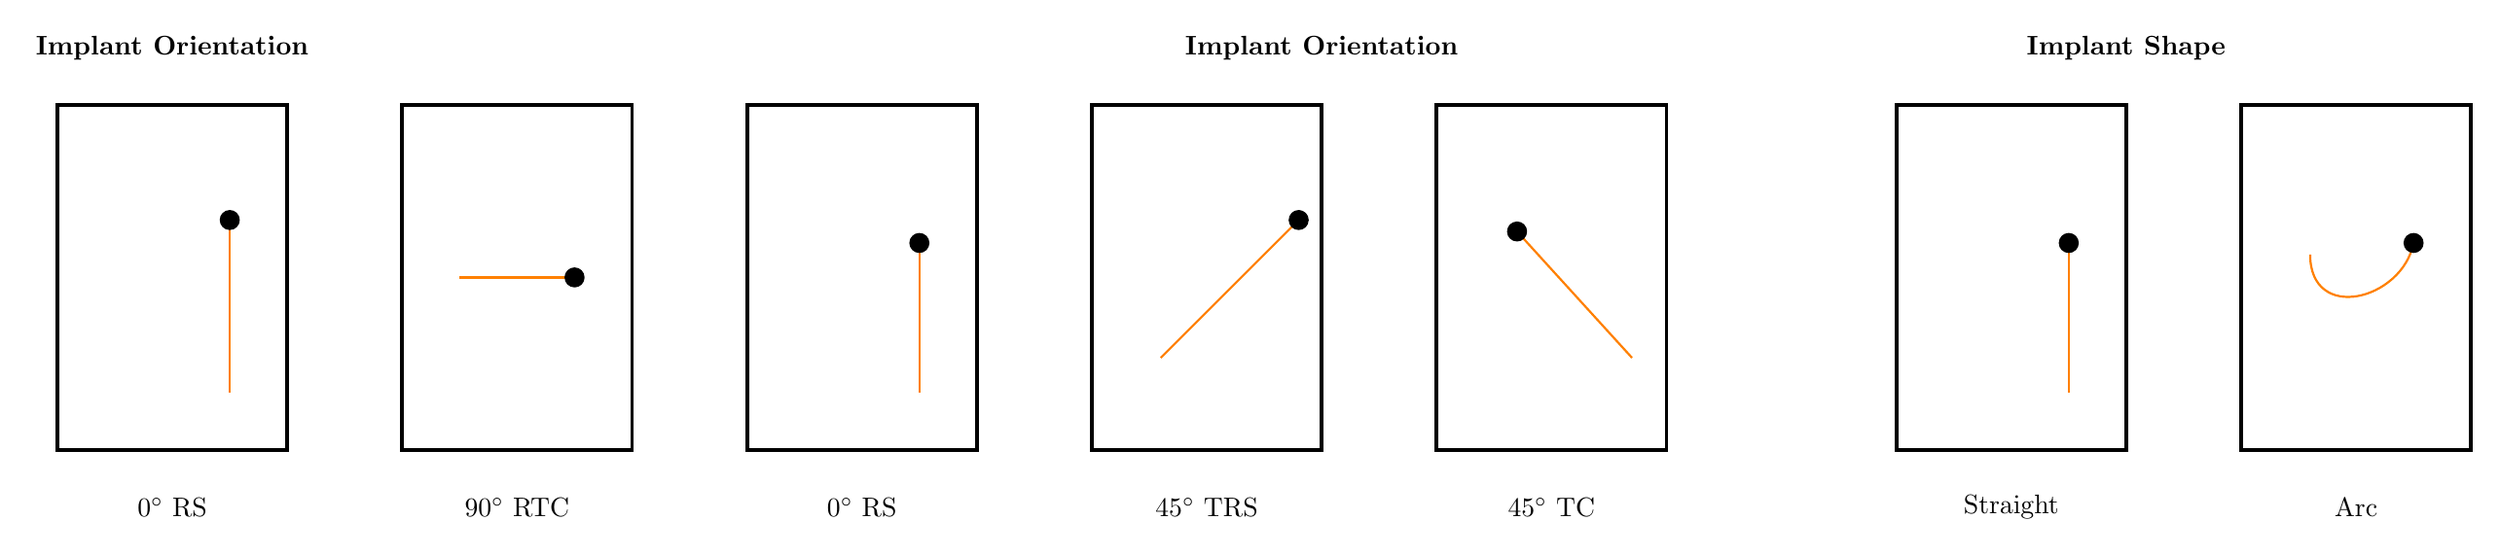
\begin{tikzpicture}[line width=0.5mm, scale=1.5]

% First Group: Implant Orientation
\node at (1, 3.5) {\textbf{Implant Orientation}};
% 0° RS
\draw[black] (0, 3) rectangle (2, 0);
\draw[orange, thick] (1.5, 2) -- (1.5, 0.5); % Adjusted position
\filldraw[black] (1.5, 2) circle (2pt);
% 90° RTC
\draw[black] (3, 3) rectangle (5, 0);
\draw[orange, thick] (3.5, 1.5) -- (4.5, 1.5); % Adjusted position
\filldraw[black] (4.5, 1.5) circle (2pt);

\node at (1, -0.5) {0$^{\circ}$ RS};
\node at (4, -0.5) {90$^{\circ}$ RTC};


% Second Group: Implant Orientation
\node at (11, 3.5) {\textbf{Implant Orientation}};
% 0° RS
\draw[black] (6, 3) rectangle (8, 0);
\draw[orange, thick] (7.5, 1.8) -- (7.5, 0.5); % Adjusted position
\filldraw[black] (7.5, 1.8) circle (2pt);
% 45° TRS
\draw[black] (9, 3) rectangle (11, 0);
\draw[orange, thick] (10.8, 2) -- (9.6, 0.8); % Refined diagonal
\filldraw[black] (10.8, 2) circle (2pt);
% 45° TC
\draw[black] (12, 3) rectangle (14, 0);
\draw[orange, thick] (12.7, 1.9) -- (13.7, 0.8); % Refined flipped diagonal
\filldraw[black] (12.7, 1.9) circle (2pt);

\node at (7, -0.5) {0$^{\circ}$ RS};
\node at (10, -0.5) {45$^{\circ}$ TRS};
\node at (13, -0.5) {45$^{\circ}$ TC};

% Third Group: Implant Shape
\node at (18, 3.5) {\textbf{Implant Shape}};
% Straight
\draw[black] (16, 3) rectangle (18, 0);
\draw[orange, thick] (17.5, 1.8) -- (17.5, 0.5); % Adjusted position
\filldraw[black] (17.5, 1.8) circle (2pt);
% Arc with V shape
\draw[black] (19, 3) rectangle (21, 0);
\draw[orange, thick] (19.6, 1.7) .. controls (19.6, 1.1) and (20.4, 1.3) .. (20.5, 1.8);
\filldraw[black] (20.5, 1.8) circle (2pt);

\node at (17, -0.5) {Straight};
\node at (20, -0.5) {Arc};

\end{tikzpicture}